\section{Příklad 1}
\prvniZadani{E}
	{
	\Large Řešení metodou postupného zjednodušování}\\

	\begin{figure}[H]
		\center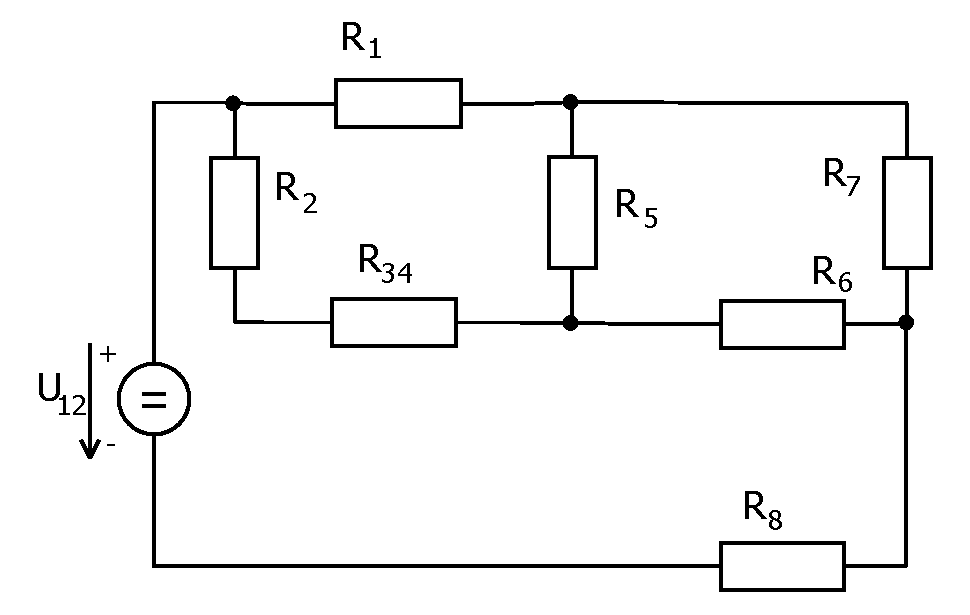
\includegraphics[width=0.6\linewidth]{obr/1_2}
		\caption{$R_3$ a $R_4$ jsou zapojeny paralelně a zdroje $U_1$ a $U_2$ sériově }
	\end{figure}
	\begin{gather*}
		R_{34} = \frac{R_3 R_4}{R_3 + R_4} =\frac{100 \cdot 340}{100 + 340} \doteq 77.2727 \Omega \\
		U_{12} = {U_1 + U_2} = {115 + 55} = 170  \text{V}
	\end{gather*}
	\begin{figure}[H]
		\center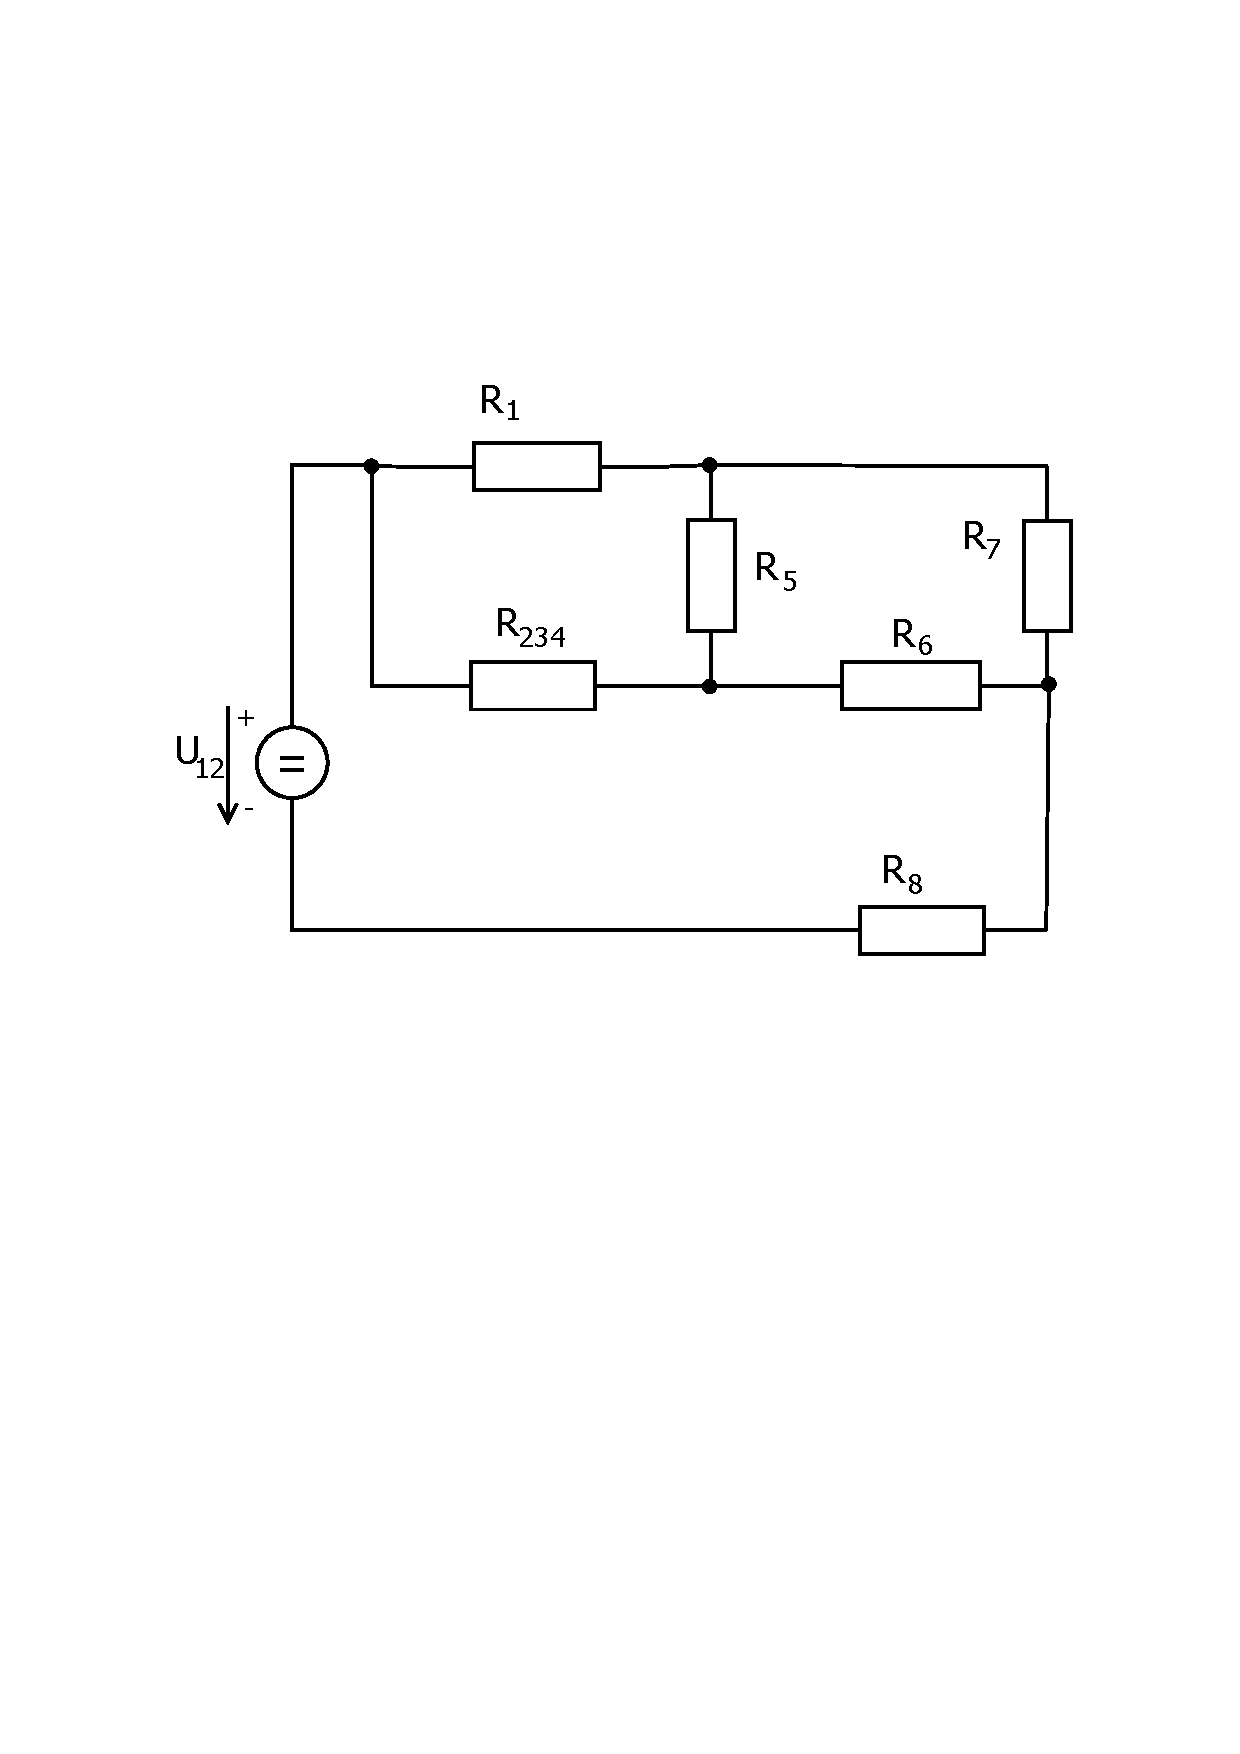
\includegraphics[width=0.6\linewidth]{obr/1_3}
		\caption{$R_2$ a $R_{34}$ jsou zapojeny sériově}
	\end{figure}
	\begin{gather*}
		R_{234} = R_2 + R_{34} = 660 + 77.2727 = 737.2727 \Omega
	\end{gather*}
	\begin{figure}[H]
		\center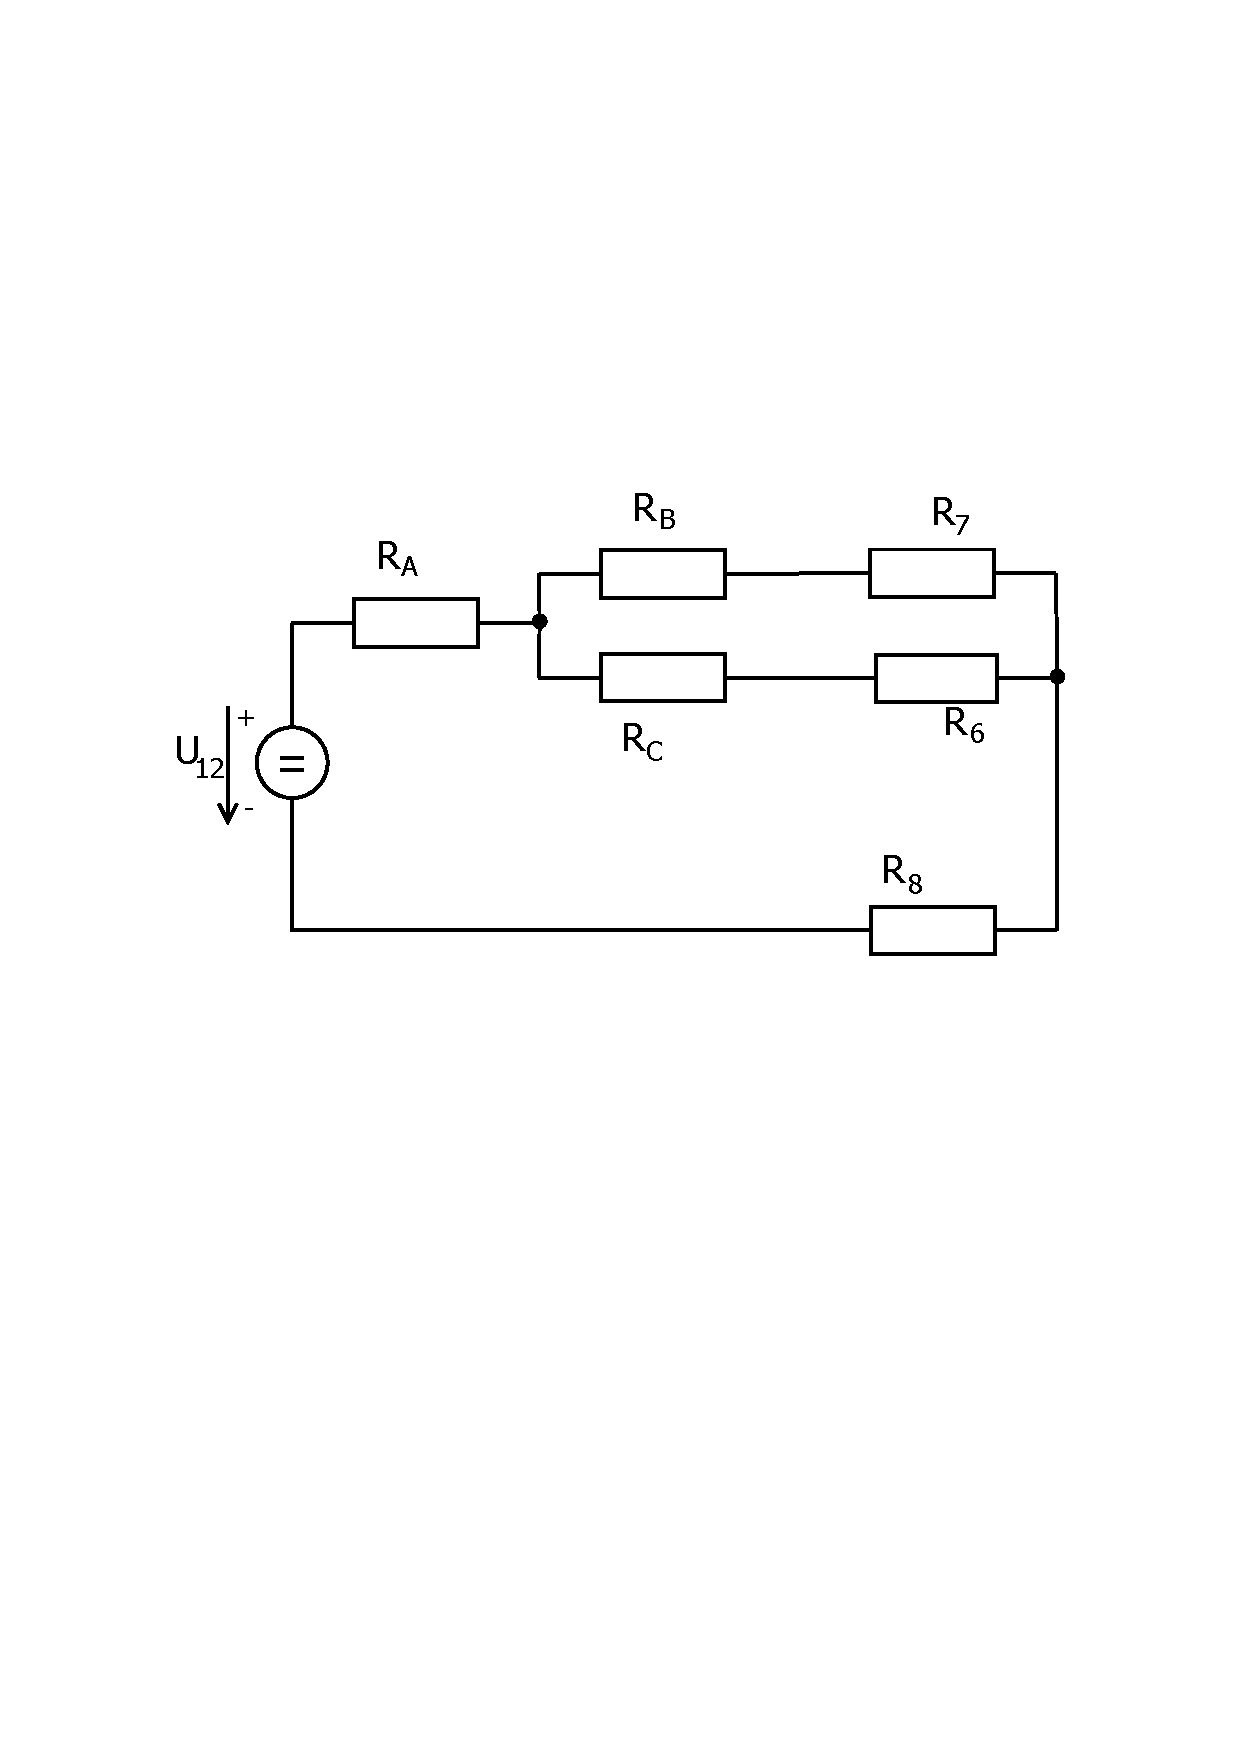
\includegraphics[width=0.6\linewidth]{obr/1_4}
		\caption{transfigurace - trojúhelník}
	\end{figure}
	\begin{gather*}
		R_A = \frac{R_1  R_{234}}{R_1 + R_{234} + R_5} = \frac{485 \cdot 737.2727}{485 +  737.2727 + 575} = 198.9555 \Omega \\
		R_B = \frac{R_1  R_5}{R_1 + R_{234} + R_5} = \frac{485 \cdot 575}{485 +  737.2727 + 575} = 155.1657 \Omega \\
		R_C = \frac{R_5  R_{234}}{R_1 + R_{234} + R_5} = \frac{575 \cdot 737.2727}{485 +  737.2727 + 575} = 235.8751 \Omega 
	\end{gather*}
	\begin{figure}[H]
		\center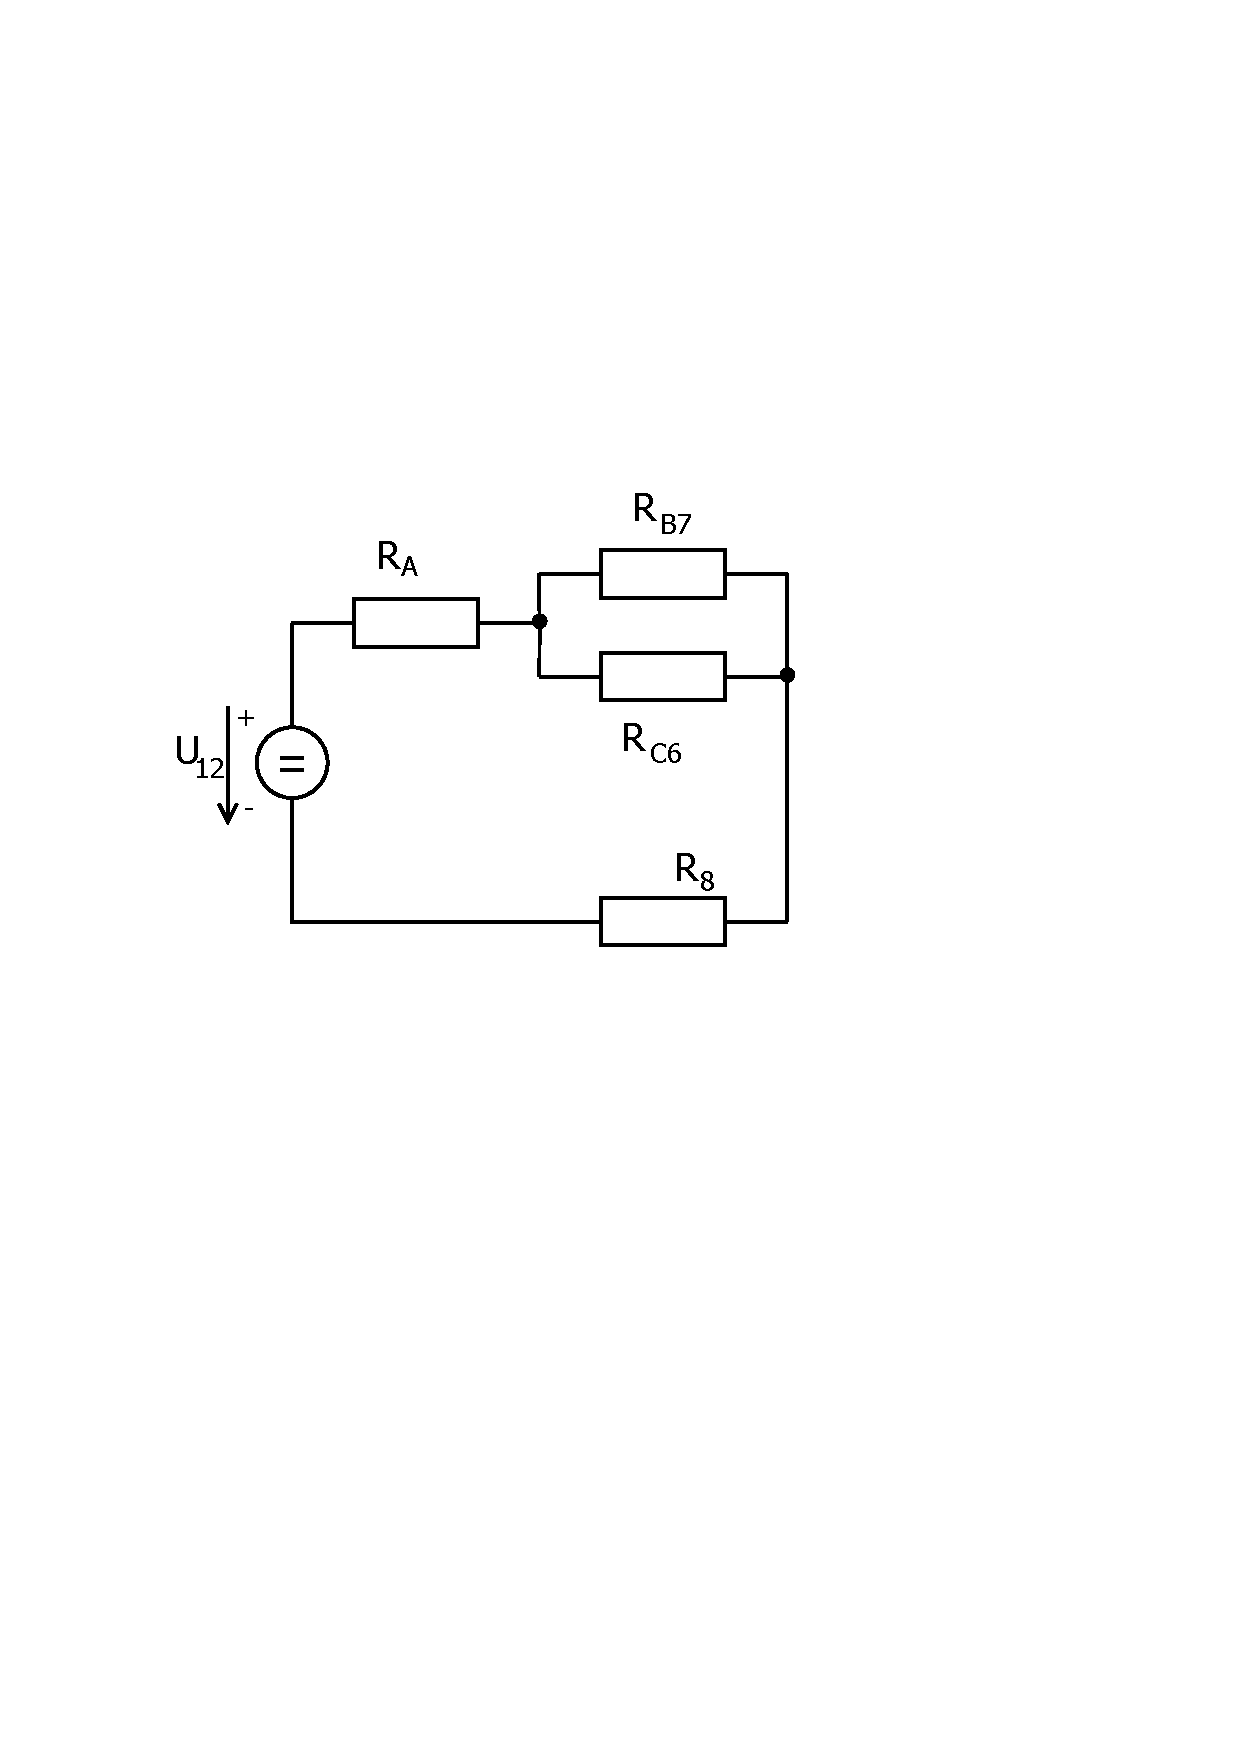
\includegraphics[width=0.6\linewidth]{obr/1_5}
		\caption{$R_B$ a $R_7$ jsou zapojeny sériově stejně jako $R_C$ a $R_6$}
	\end{figure}
	\begin{gather*}
		R_{B7} = R_B + R_7 = 155.1657 + 255 = 410.1657 \Omega \\
		R_{C6} = R_C + R_6 =235.8751 + 815 = 1050,8751 \Omega
	\end{gather*}
	\begin{figure}[H]
		\center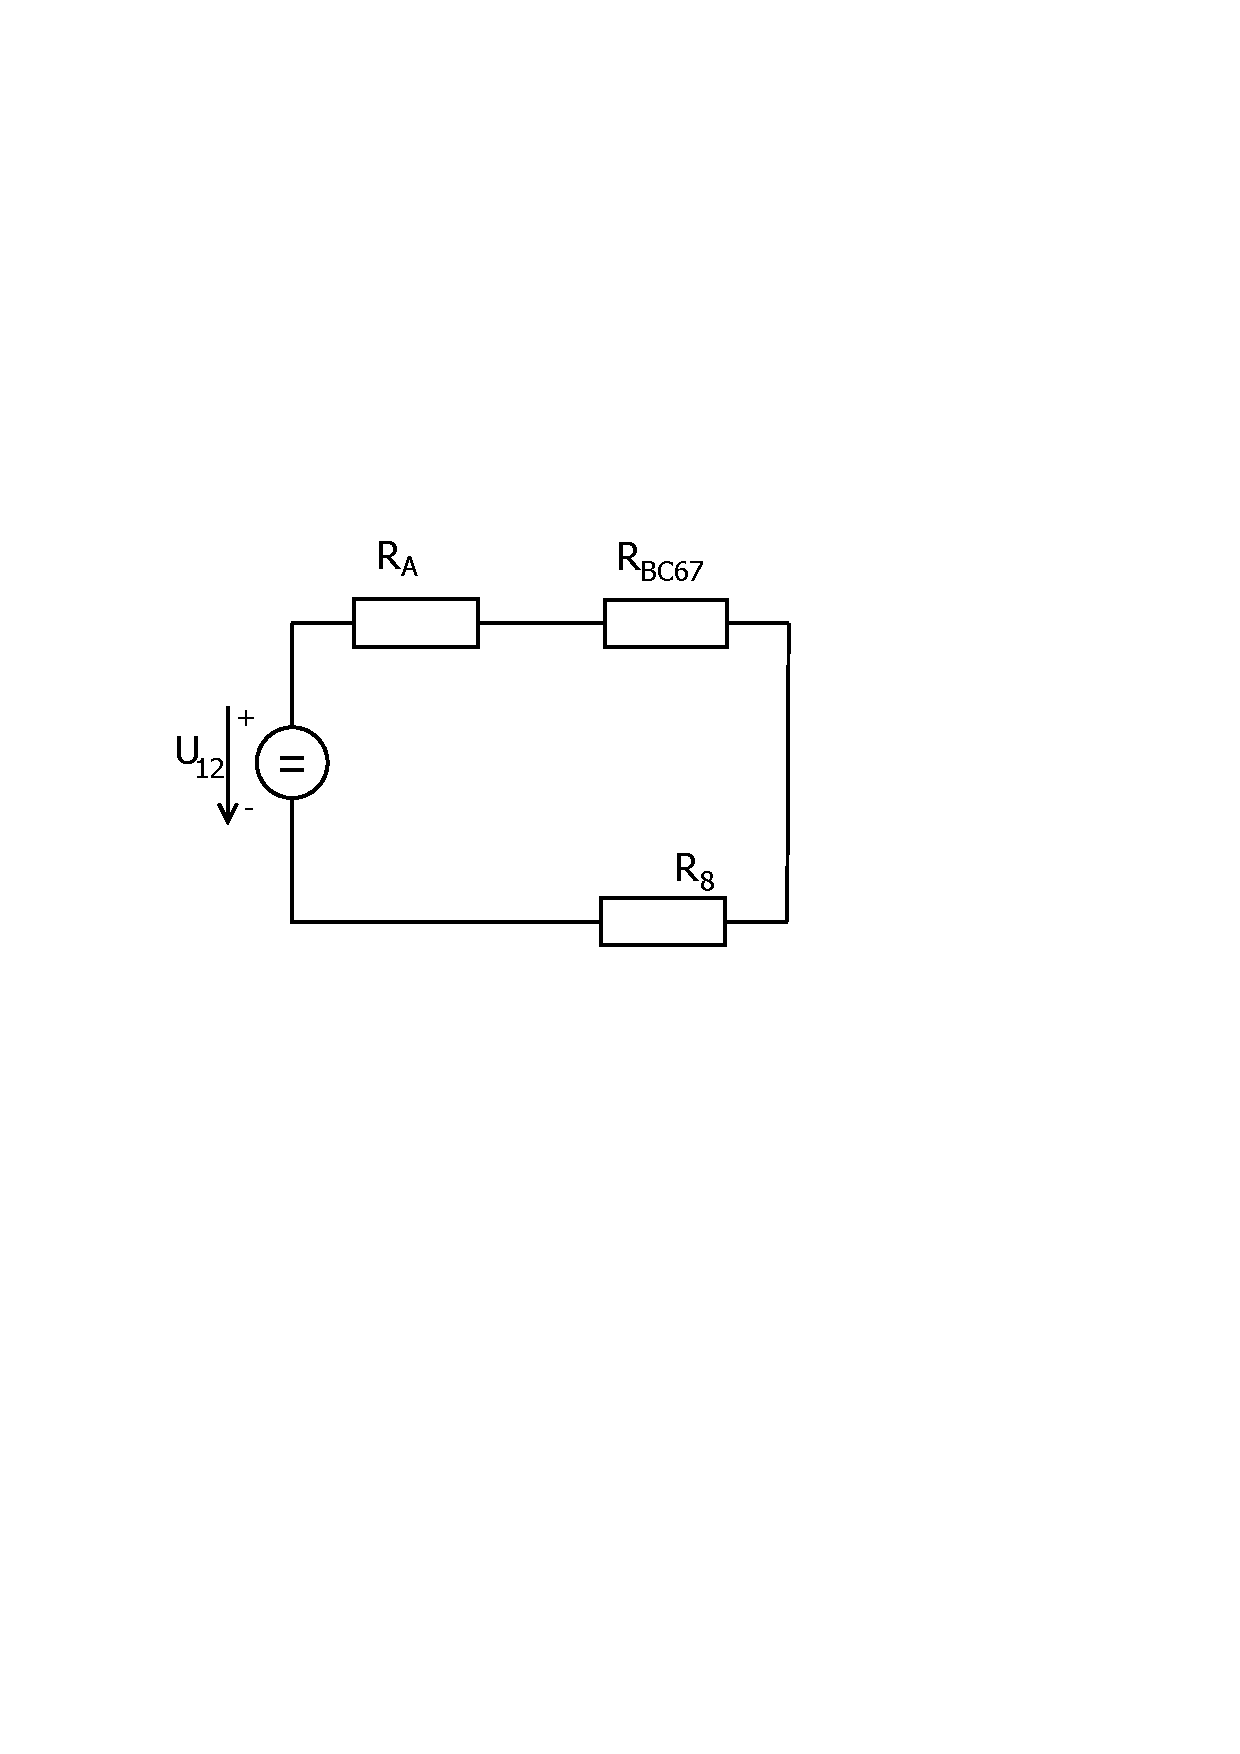
\includegraphics[width=0.6\linewidth]{obr/1_6}
		\caption{ $R_{B7}$ a $R_{C6}$ jsou zapojeny paralelně}
	\end{figure}
	\begin{gather*}
		R_{BC67} = \frac{R_{B7} R_{C6}}{R_{B7} + R_{C6}} = \frac{410.1657 \cdot 1050,8751}{410.1657 + 1050,8751} = 295.0177 \Omega
	\end{gather*}

	\begin{figure}[H]
		\center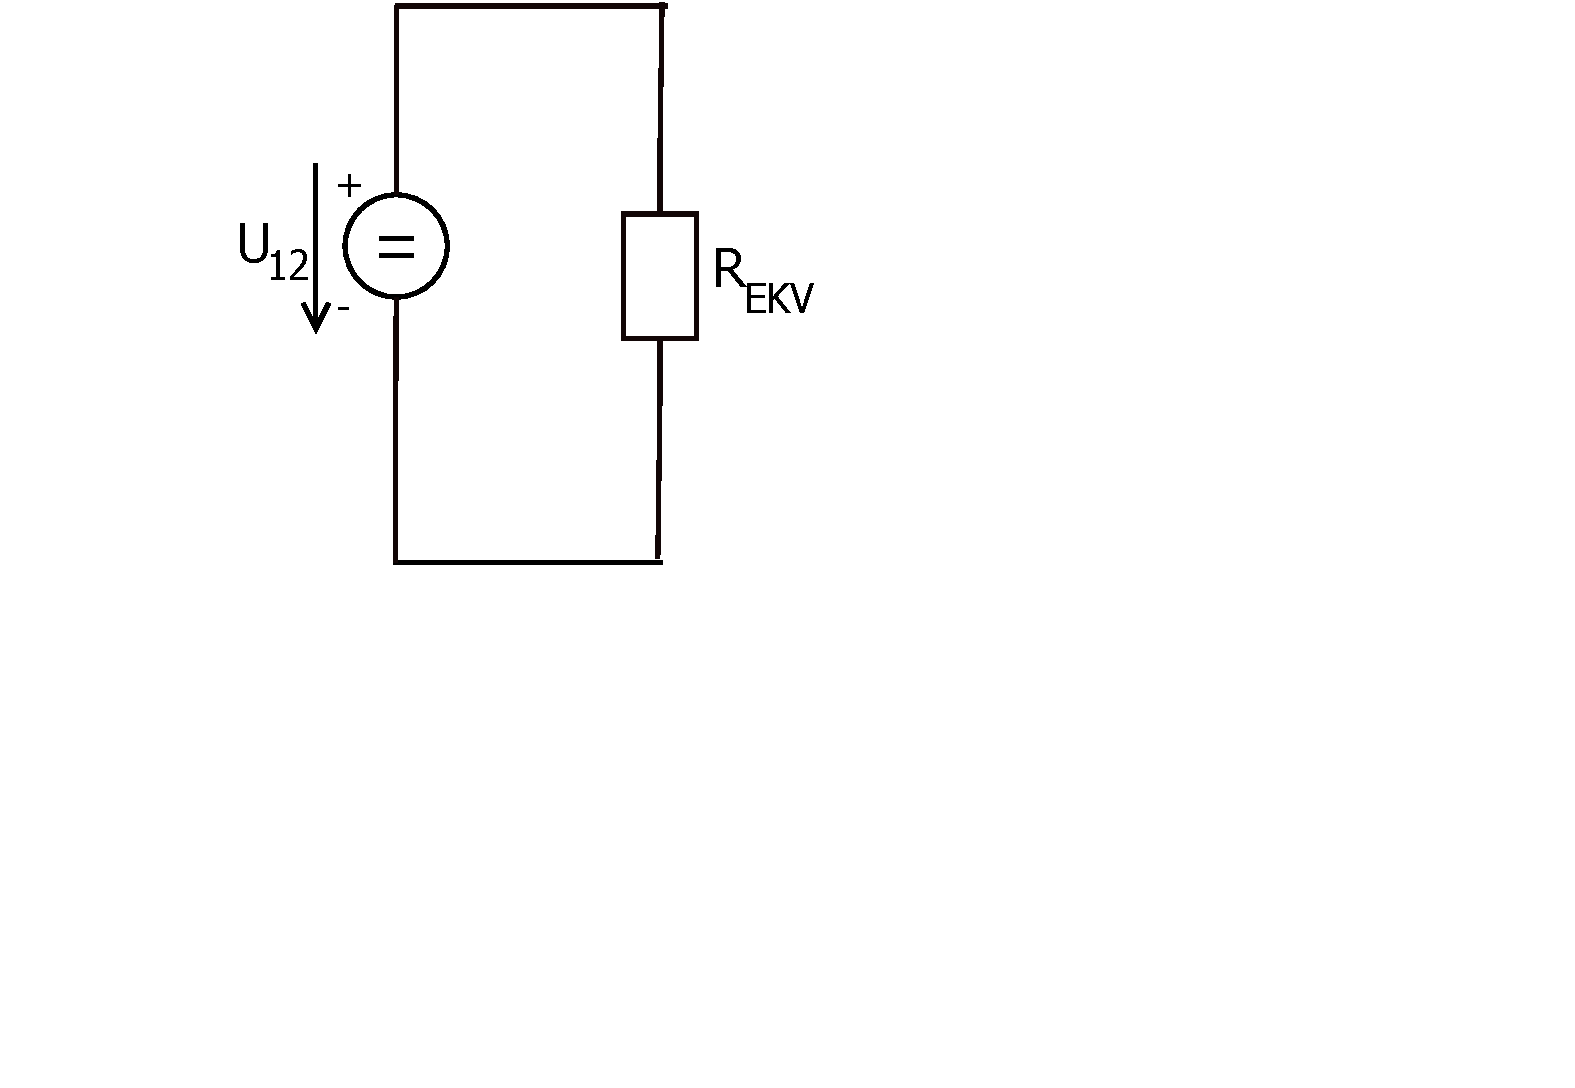
\includegraphics[width=0.3\linewidth]{obr/1_7}
		\caption{$R_A$ a $R_{BC67}$ a $R_8$ jsou zapojeny sériově - získáváme $R_{EKV}$}
	\end{figure}
	\begin{gather*}
		R_{EKV} = R_{A} + R_{BC67} + R_8 = 198.9555 + 295.0177 + 225 = 718.9732 \Omega
	\end{gather*}

	Celkový proud $I$:
	\begin{gather*}
		I = \frac{U_{12}}{R_{EKV}} = \frac{170}{718.9732} \doteq 0,2364 \text{A}
	\end{gather*}

	Začneme zpětně počítat napětí a proudy, až dojdeme k $U_{R_6}$ a $I_{R_6}$:

	\begin{figure}[H]
		\center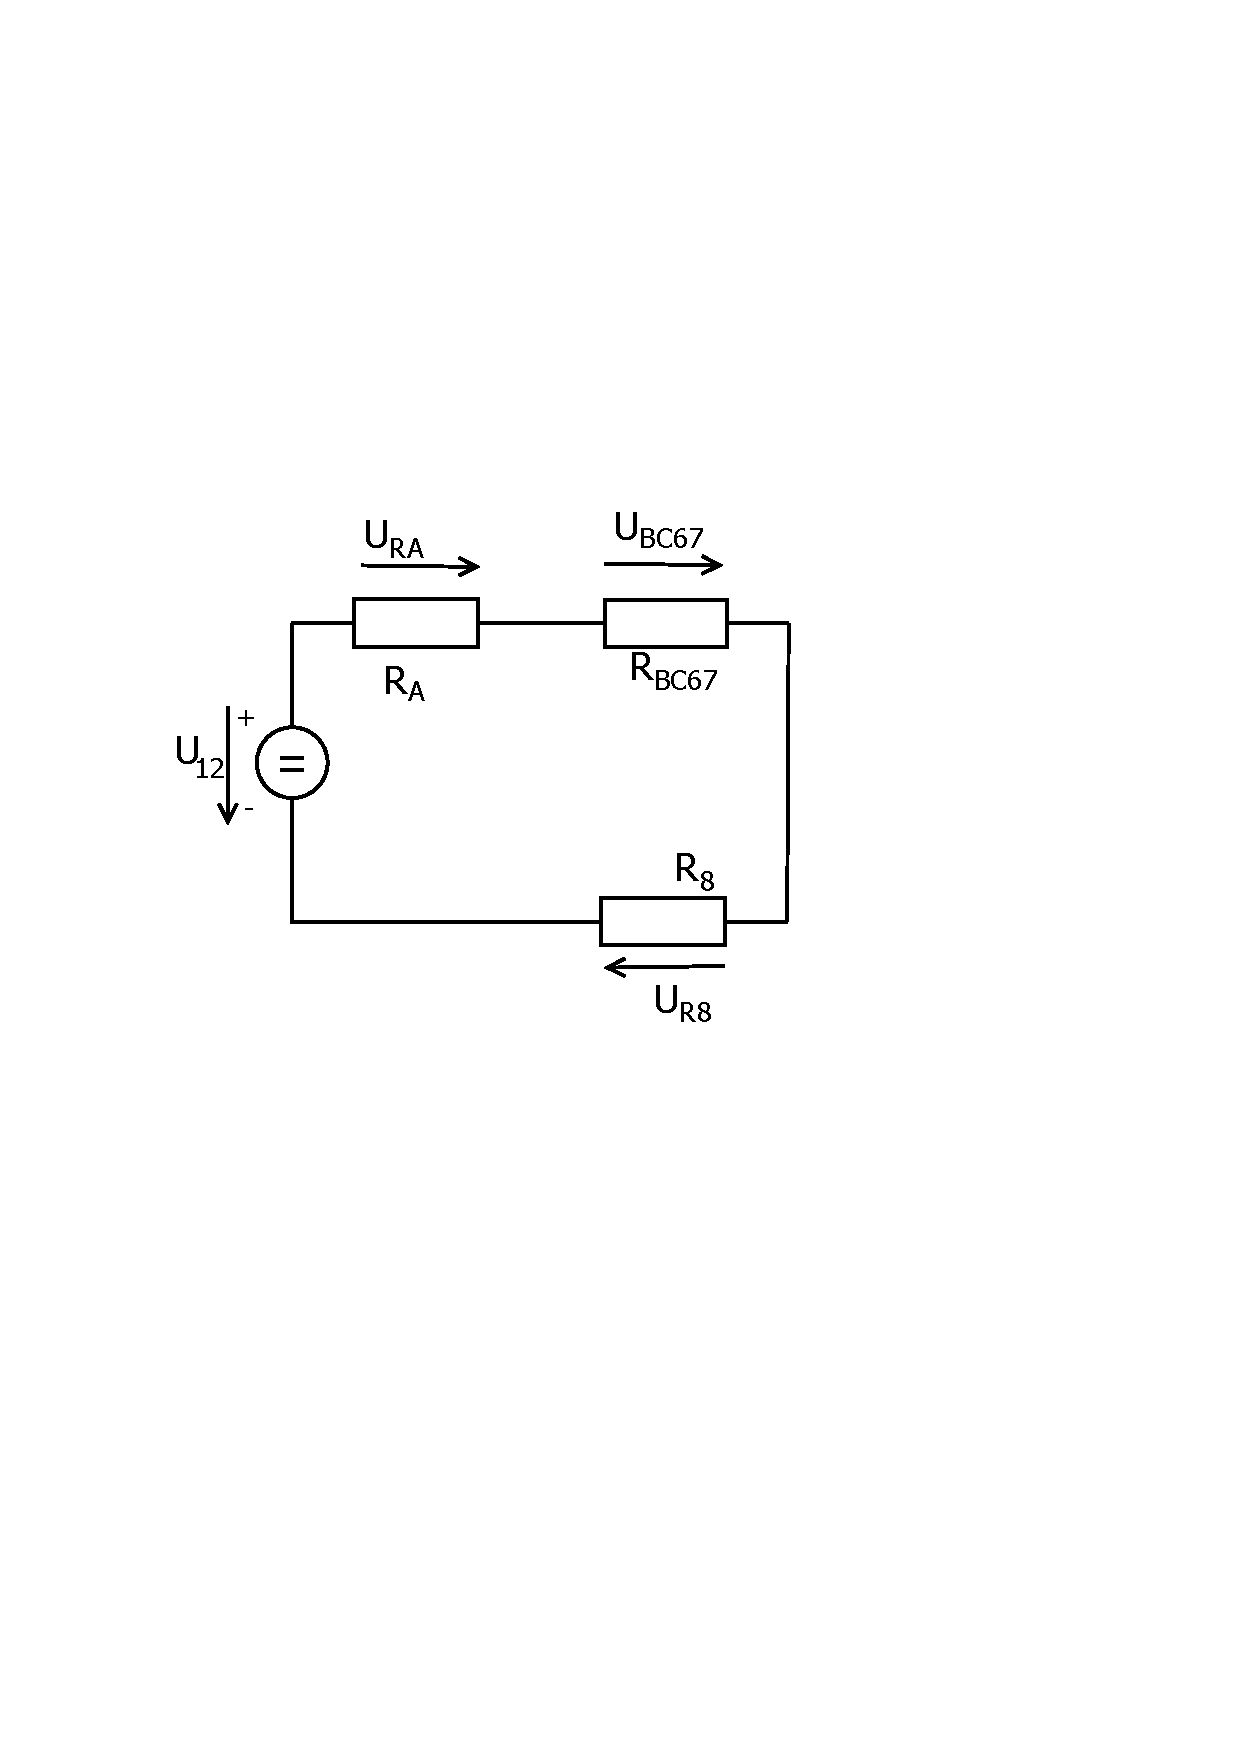
\includegraphics[width=0.6\linewidth]{obr/1_8}
		\caption{Spočítáme si napětí na jednotlivých odporech}
	\end{figure}
	\begin{gather*}
		U_{R_A} = {I R_A} = {0,2364\cdot 198.9555} \doteq 47.0331  \text{V} \\
		U_{R_{BC67}} = {I R_{BC67}} = {0,2364 \cdot 295.0177} \doteq 69.7422  \text{V} \\
		U_{R_8} = {I R_8} = {0,2364 \cdot 225} = 53.19  \text{V} \\
		\\
		\text{Provedeme kontrolu pomocí II. Kirchhoffova zákona.}  \\
		U_{R_A} + U_{R_{BC67}} + U_{R_8} - U_{12} =  0 \\
	\end{gather*}

	\begin{figure}[H]
		\center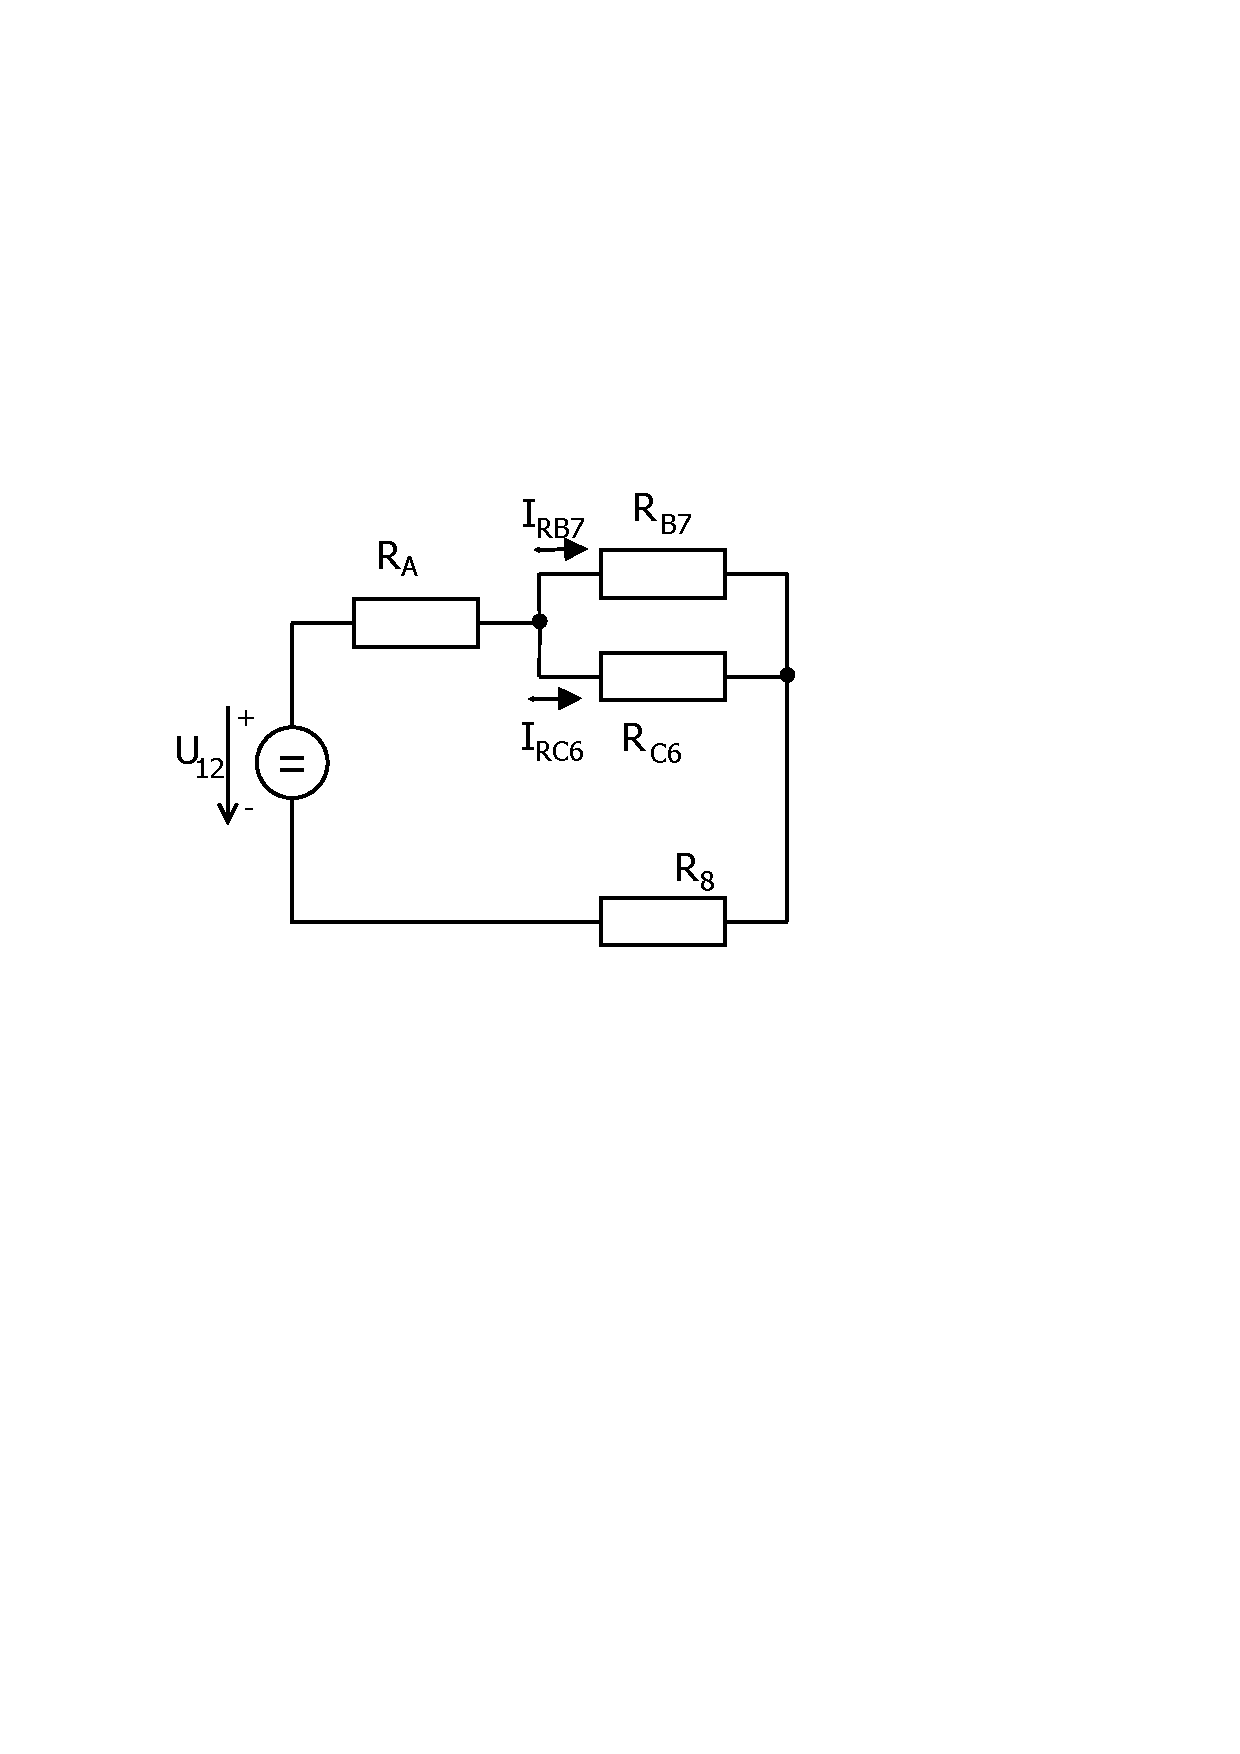
\includegraphics[width=0.6\linewidth]{obr/1_9}
		\caption{Spočítáme si proud ve větvích s $R_{B7}$ a  $R_{C6}$}
	\end{figure}
	\begin{gather*}
		I_{R_{B7}} = \frac{U_{R_{BC67}}{R_{B7}}} = \frac{69.7422}{410.1657} \doteq 0,17 \text{A} \\
		I_{R_{C6}} = \frac{U_{R_{BC67}}{R_{C6}}} = \frac{69.7422}{1050,8751} \doteq 0.0664 \text{A} \\
		\\
		\text{Provedeme kontrolu pomocí I. Kirchhoffova zákona.}  \\
		I_{R_{B7}} + I_{R_{C6}} - I  =  0 
	\end{gather*}

	\begin{figure}[H]
		\center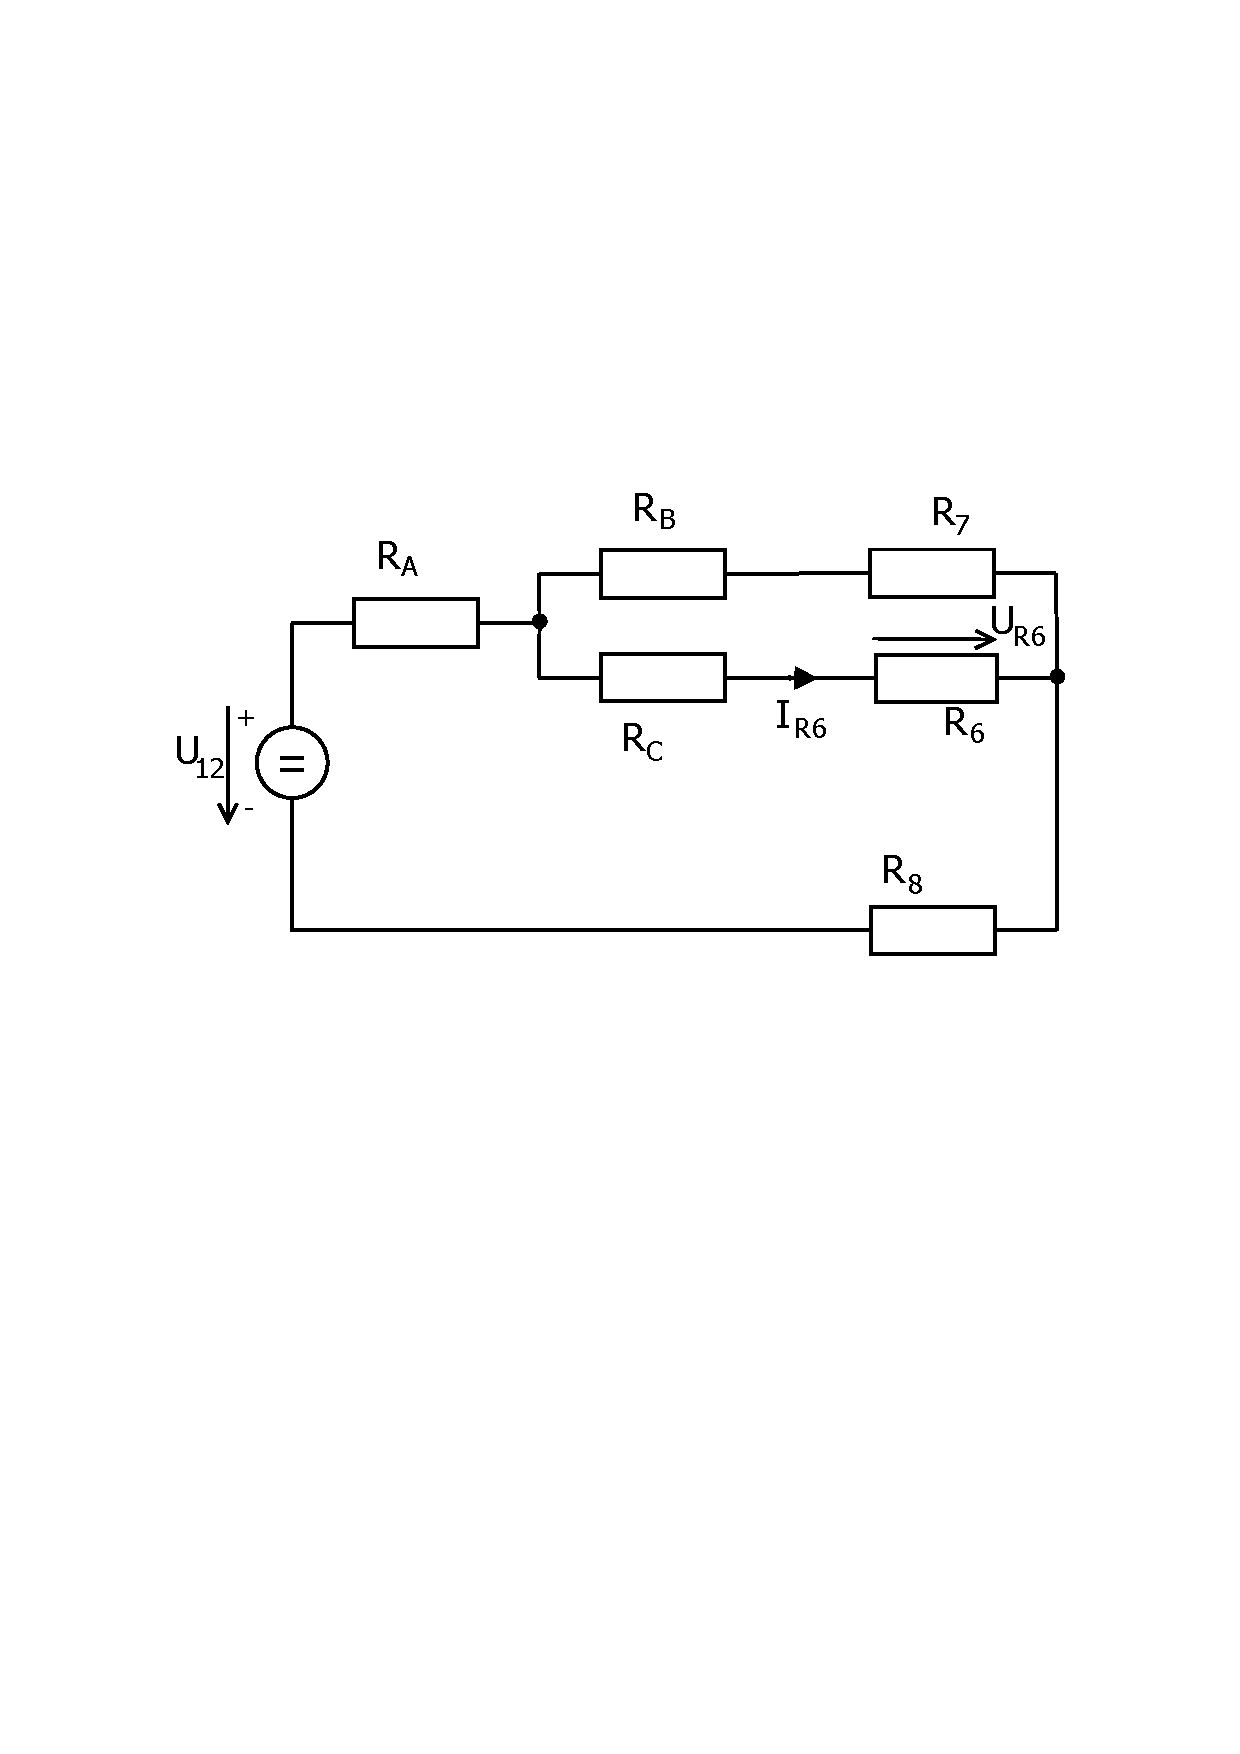
\includegraphics[width=0.6\linewidth]{obr/1_10}
		\caption{Spočítáme si napětí a proud u $R_6$}
	\end{figure}
	\begin{gather*}
		I_{R_{C6}} = I_{R_6} = 0.0664 \text{A} \\
		U_{R_6} = {I_{R_6} R_6} = {0.0664 \cdot 815} = 54.116  \text{V} \\
	\end{gather*}